% Created 2012-09-04 Tue 00:28
\documentclass[11pt]{article}
\usepackage[utf8]{inputenc}
\usepackage[T1]{fontenc}
\usepackage{fixltx2e}
\usepackage{graphicx}
\usepackage{longtable}
\usepackage{float}
\usepackage{wrapfig}
\usepackage{soul}
\usepackage{textcomp}
\usepackage{marvosym}
\usepackage{wasysym}
\usepackage{latexsym}
\usepackage{amssymb}
\usepackage{hyperref}
\tolerance=1000
\providecommand{\alert}[1]{\textbf{#1}}

\title{Waliji Experiments}
\author{Mark Stoehr}
\date{\today}
\hypersetup{
  pdfkeywords={},
  pdfsubject={},
  pdfcreator={Emacs Org-mode version 7.8.11}}

\begin{document}

\maketitle

\setcounter{tocdepth}{3}
\tableofcontents
\vspace*{1cm}
\section{Notation}
\label{sec-1}

\begin{itemize}
\item $\pi_k$ is a mixture weight
\item $e$ is an index for the edge orientation
\item $t,s$ are time indices
\item $f$ is a frequency band
\item $X\in \{0,1\}^{|\{e\}|,|\{f\}|,|\{s\}|}$ is the output of our edge
    detector ranging over edge locations $|\{e\}|$, frequency bands
    $|\{f\}|$, and time indices $|\{s\}|$
\item $X_{e,f,s}$ is a given binary variable for whether an edge is
    detected at $(e,f,s)$ in the collection denoted by $X$ and
    $X_{i,e,f,s}$ is functions in the same role for a data point $X_i$.
\item $X$ denotes the random variable, $x$ denotes the realized value
\item $[n]=\{1,\ldots,n\}$
\end{itemize}
\section{Reproduce Waliji Parts}
\label{sec-2}

Reproducing the work from the Masters thesis
\subsection{Sample work through}
\label{sec-2-1}



\begin{verbatim}
import matplotlib.pyplot as plt
import numpy as np
s = np.load('../data/1s.npy')
t = np.arange(len(s))/16.
plt.plot(t,s)
plt.xlabel('time (ms)')
plt.savefig('1s.png')
\end{verbatim}

\begin{figure}[htb]
\centering
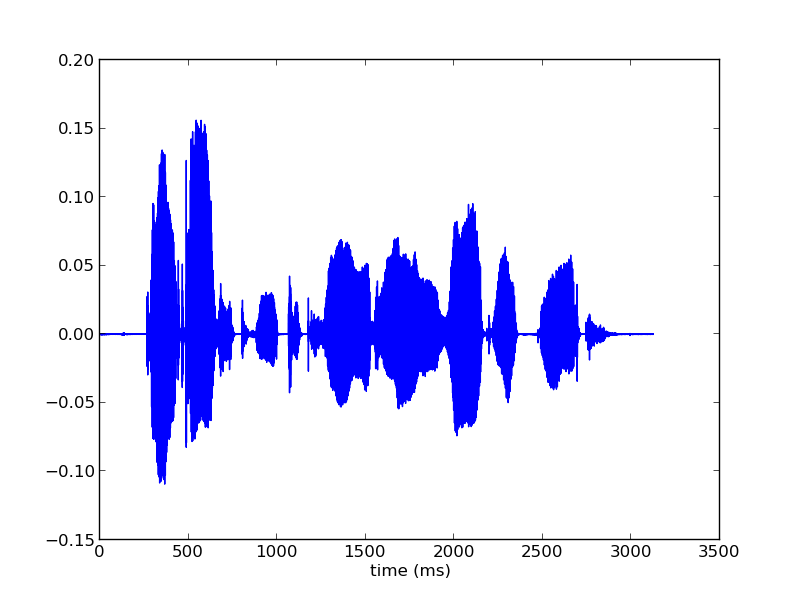
\includegraphics[height=10cm]{./1s.png}
\caption{\label{fig:1s}Example utterance waveform}
\end{figure}

We then turn this into a spectrogram.  There are two ways of doing this
the first is to use the same signal processing the Alexey Koloydenko
and Partha Niyogi developed




\begin{verbatim}
import matplotlib.pyplot as plt
import numpy as np
S = np.load('../data/1S.npy')
plt.imshow(S[::-1],interpolation='nearest',aspect=3)
plt.xticks(np.arange(7)*100,tuple(str(i*100/5) for i in xrange(7)))
# since 8*16000 (sample rate)/512 (fft length) = 250
plt.yticks(np.arange(6)*8,tuple(str(i*250) for i in xrange(6))[::-1])
plt.xlabel('time (ms)')
plt.ylabel('freq (Hz)')
plt.savefig('1S.png')
\end{verbatim}


\begin{figure}[htb]
\centering
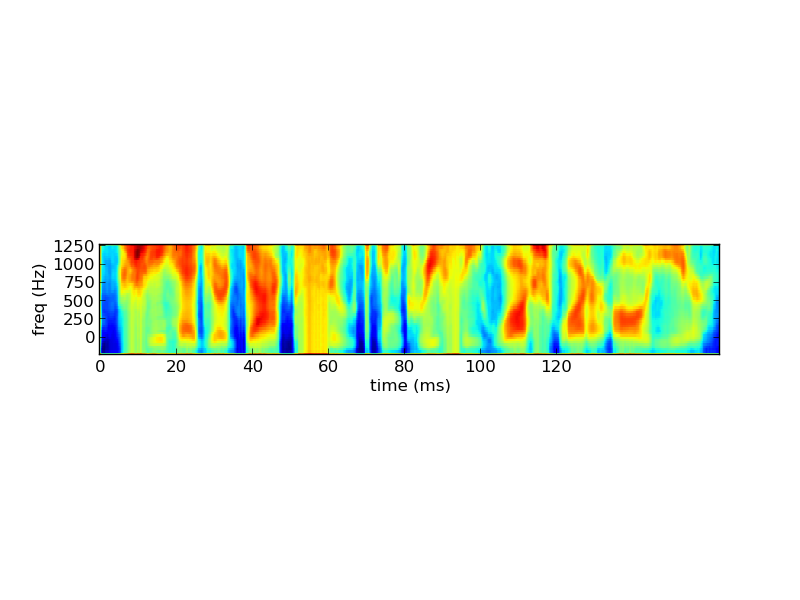
\includegraphics[height=10cm]{./1S.png}
\caption{\label{fig:1S}Example utterance Spectrogram}
\end{figure}

We can also redo this entirely as the mel spectrogram.  More on that later.

We aim to extract edge features.  The edge features we compute are done
with binary masks of the following sort


\begin{verbatim}
import matplotlib.pyplot as plt
import matplotlib.cm as cm
import numpy as np
edge_orientations = np.load('../data/edge_orientations.npy')
fig = plt.figure()
for i in xrange(8):
    plt.subplot(4,2,i+1)
    mask_mat = np.zeros((2,2))
    y_coord, x_coord = edge_orientations[i].astype(int)
    y = (y_coord +1)/2
    x = (x_coord + 1)/2
    if y_coord == 0:
        plus_one_locs = [[0,1],[x,x]]
        minus_one_locs = [[0,1],[(x + 1) %2, (x+1) %2]]
    elif x_coord == 0:
        plus_one_locs = [[y,y],[0,1]]
        minus_one_locs = [[(y+1) % 2,(y+1) %2],[0,1]]
    else:
        plus_one_locs = [[y],[x]]
        minus_one_locs = [[(y+1) % 2],[(x+1) %2]]
    mask_mat[plus_one_locs] = 1
    mask_mat[minus_one_locs] = -1
    plt.imshow(mask_mat,interpolation='nearest',
               cmap=cm.bone)
    plt.title('Edge orientation %d' % (i+1))
    frame = plt.gca()
    frame.axes.get_xaxis().set_visible(False)
    frame.axes.get_yaxis().set_visible(False)

plt.subplots_adjust(hspace=.5)
plt.savefig('edge_orientations_pic.png')
\end{verbatim}

These are represented in the following picture \ref{fig:edge_orientations}.

\begin{figure}[htb]
\centering
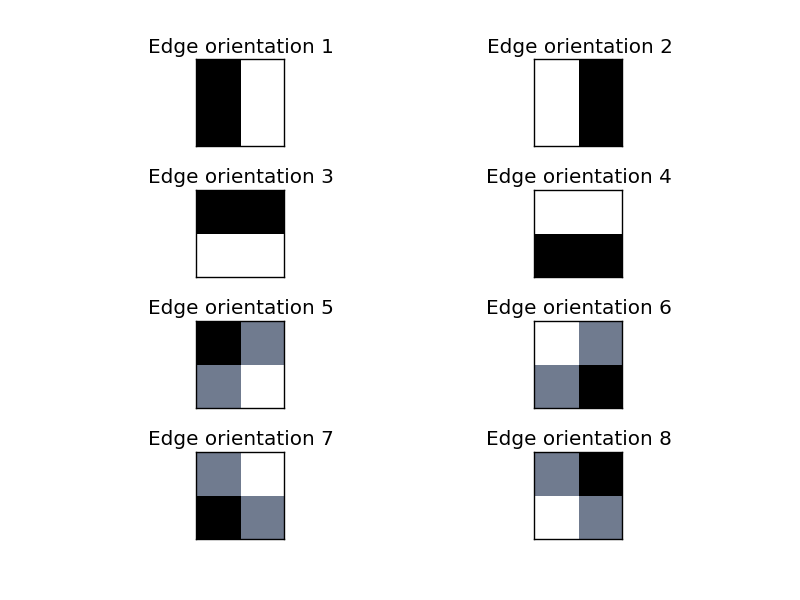
\includegraphics[height=8cm]{./edge_orientations_pic.png}
\caption{\label{fig:edge_orientations}Edge filters}
\end{figure}

Applying those filters to the image and then thresholding the outputs
we get the following edge map representation:


\begin{verbatim}
import matplotlib.pyplot as plt
import matplotlib.cm as cm
import numpy as np
E = np.load('../data/1E.npy')
plt.imshow(E[::-1],interpolation='nearest',
               cmap=cm.bone)
plt.title('Edge Map Representation')
plt.xticks(np.arange(7)*100,tuple(str(i*100/5) for i in xrange(7)))
# since 8*16000 (sample rate)/512 (fft length) = 250
plt.yticks(np.arange(8)*48 + 24,tuple(str(i+1) for i in xrange(8))[::-1])
plt.xlabel('time (ms)')
plt.ylabel('freq (Hz)')
plt.savefig('edge_map.png')
\end{verbatim}

\begin{figure}[htb]
\centering
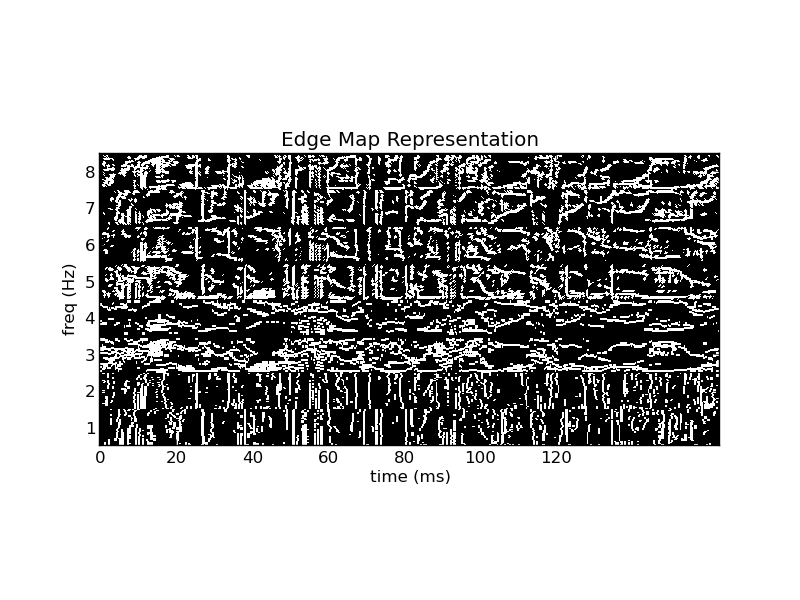
\includegraphics[height=10cm]{./edge_map.png}
\caption{\label{fig:edge_map}Edge Map Representation}
\end{figure}

In \ref{fig:edge_map} the light areas indicate where edges have been
detected. Also bear in mind that we spread the edges.  Since there are
eight orientations to the edges each edge filter produces a separate
copy of the spectrogram.  We stacked these representations onto the
same figure and the y-axis consists of blocks of these
representation. Increasing along the y-axis are the frequency locations.

We then extract features related to 6 by 6 square patches in the
spectrogram.  These features are associated with an 8 by 5 by 5 patch
of the edge map, where we have a 5 by 5 patch from each edge map
associated with a particular edge orientation.  We only consider such
patches if the number of edges is above a certain threshold: chosen to 
be the 90th percentile following Waliji.

In the particular example above we have 21120 total patches and the
distribution over the number of edges is given in
\ref{fig:edge_count_histogram} and the cutoff point is at about 70
edges.  Each patch can have potentially 200 edges in it (although its
impossible for a signal to have that many edges).


\begin{verbatim}
import matplotlib.pyplot as plt
import matplotlib.cm as cm
import numpy as np
bp_all = np.load('../data/1bp_all.npy')
plt.close()
plt.hist(bp_all.sum(1).sum(1))
plt.title('Histogram over number of edges in given patches')
plt.savefig('edge_count_patches_histogram.png')
plt.close()
\end{verbatim}


\begin{figure}[htb]
\centering
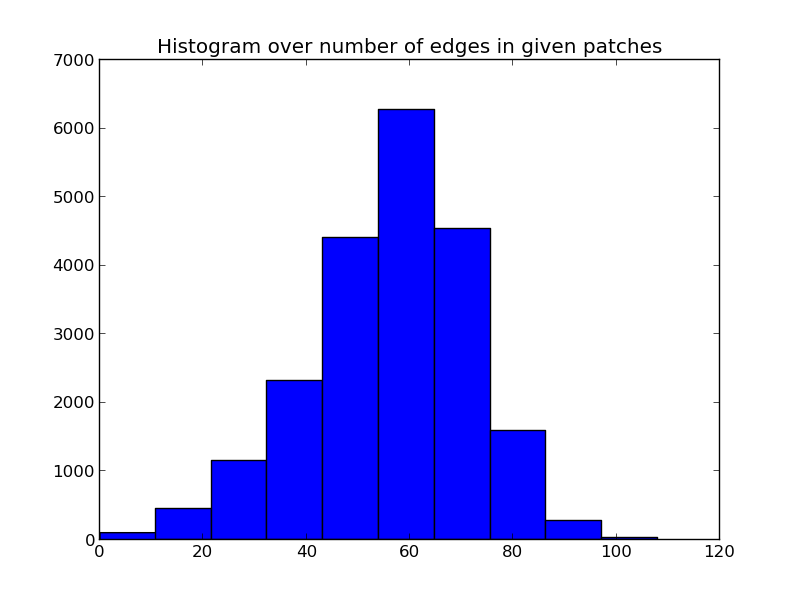
\includegraphics[height=10cm]{./edge_count_patches_histogram.png}
\caption{\label{fig:edge_count_histogram}Patch Edge Count Histogram}
\end{figure}

We see that the number of edges in a patch is approximately normal.
We can then look at the spectrogram patches that are associated with these
edgemap patches.  


\begin{verbatim}
import matplotlib.pyplot as plt
import matplotlib.cm as cm
import numpy as np
from sklearn import mixture

spec_patch = np.load('../data/1spec_patch.npy')
spec_patch_flat = spec_patch.reshape(spec_patch.shape[0],6*6)
for i in [1,2,3,5,8,13,21]:
    clf = mixture.GMM(n_components=i,n_init=10)
    clf.fit(spec_patch_flat)
    num_rows = i/3+1
    if i < 3:
        num_cols = i+1
    else:
        num_cols = 3
    fig = plt.figure()
    plt.title('Mixture Components')
    for j in xrange(i):
        plt.subplot(num_rows,num_cols,j+1)
        plt.imshow(clf.means_[j].reshape(6,6),
                   cmap=cm.bone)
        frame = plt.gca()
        frame.axes.get_xaxis().set_visible(False)
        frame.axes.get_yaxis().set_visible(False)
    plt.savefig('spec_patch_clustersGMM%d.png' % i)
\end{verbatim}


\begin{figure}[htb]
\centering

\includegraphics[height=10cm]{./spec_patch_clustersGMM1.png}
\caption{\label{fig:spec_patch_clustersGMM1}Spectrogram Patch Mean}
\end{figure}

\begin{figure}[htb]
\centering
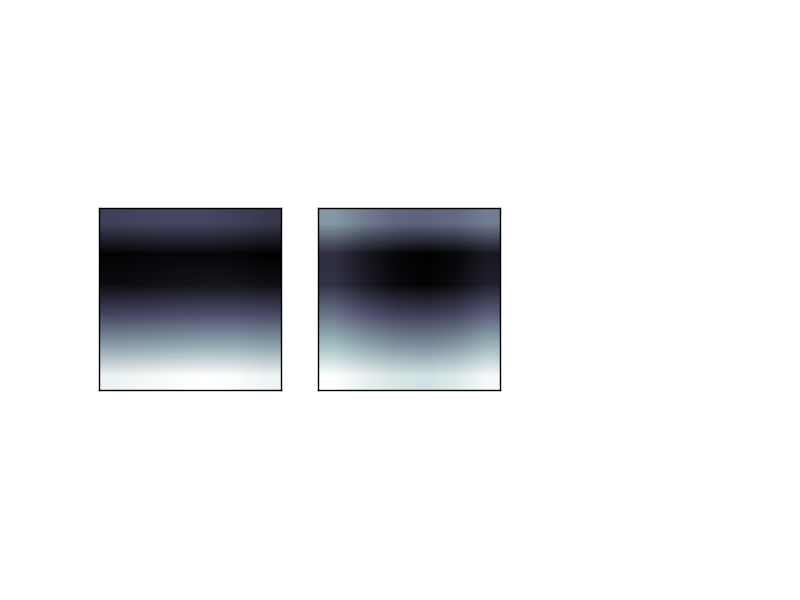
\includegraphics[height=10cm]{./spec_patch_clustersGMM2.png}
\caption{\label{fig:spec_patch_clustersGMM2}Spectrogram Patch GMM - 2 Clusters}
\end{figure}


\begin{figure}[htb]
\centering
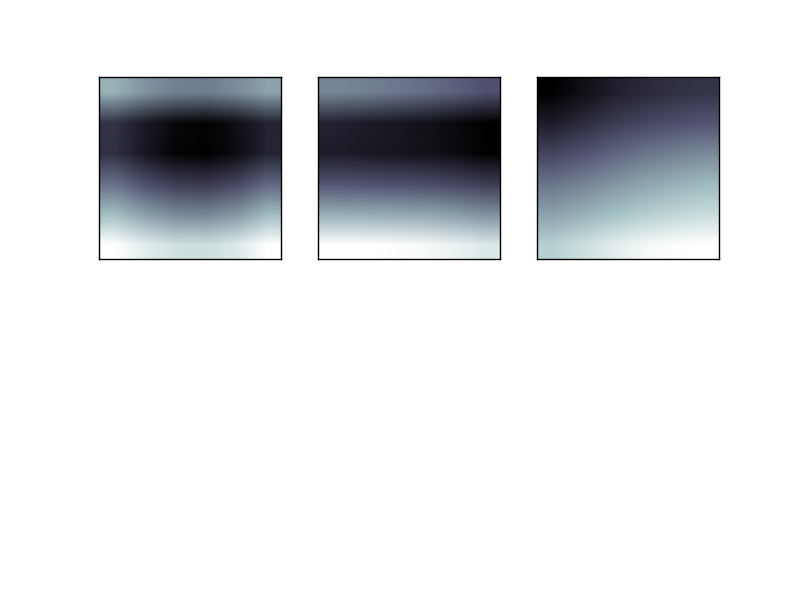
\includegraphics[height=10cm]{./spec_patch_clustersGMM3.png}
\caption{\label{fig:spec_patch_clustersGMM3}Spectrogram Patch GMM - 3 Clusters}
\end{figure}


\begin{figure}[htb]
\centering
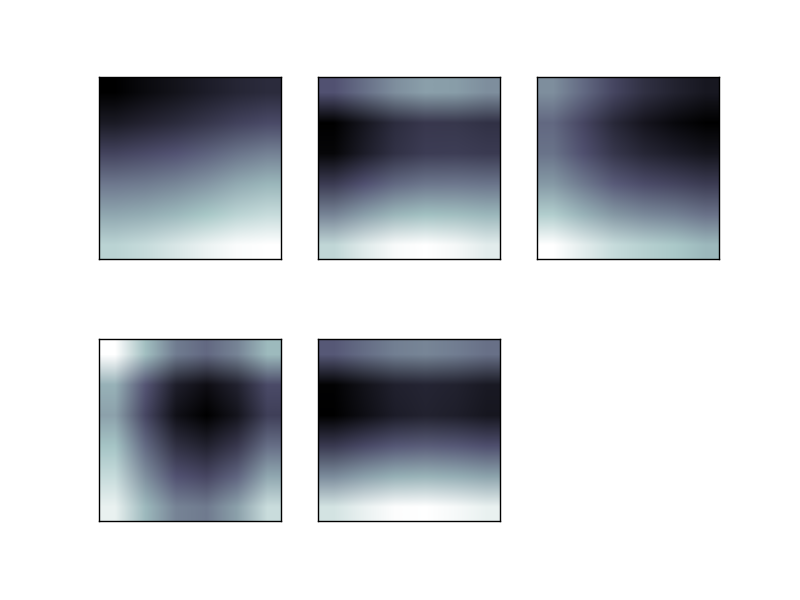
\includegraphics[height=10cm]{./spec_patch_clustersGMM5.png}
\caption{\label{fig:spec_patch_clustersGMM5}Spectrogram Patch GMM - 5 Clusters}
\end{figure}


\begin{figure}[htb]
\centering
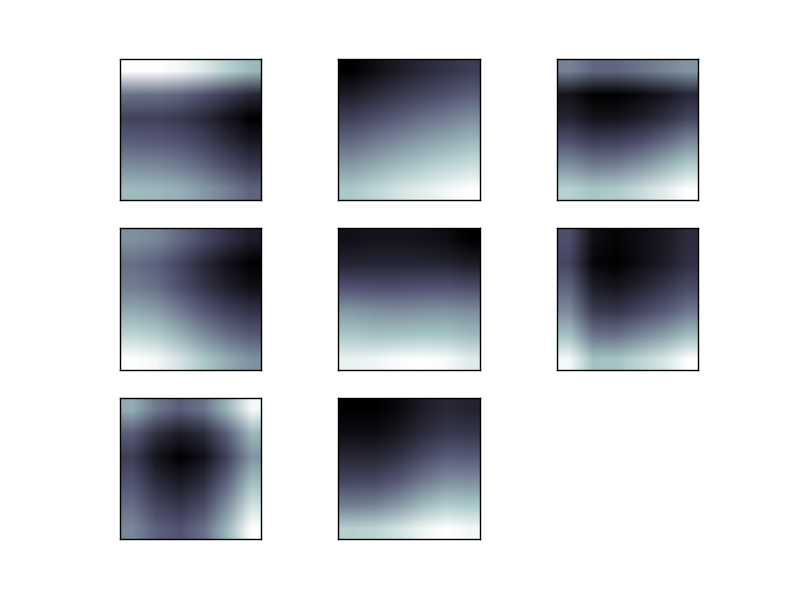
\includegraphics[height=10cm]{./spec_patch_clustersGMM8.png}
\caption{\label{fig:spec_patch_clustersGMM8}Spectrogram Patch GMM - 8 Clusters}
\end{figure}

\begin{figure}[htb]
\centering
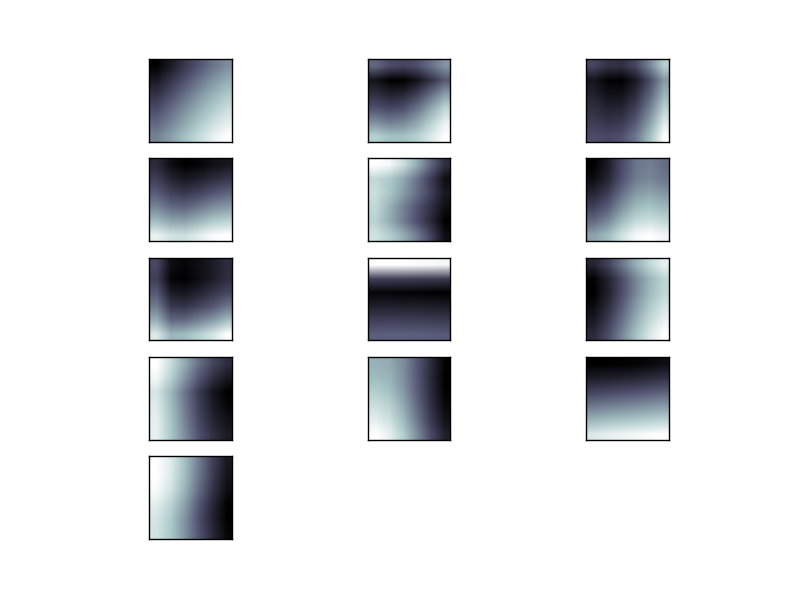
\includegraphics[height=10cm]{./spec_patch_clustersGMM13.png}
\caption{\label{fig:spec_patch_clustersGMM13}Spectrogram Patch GMM - 13 Clusters}
\end{figure}

\begin{figure}[htb]
\centering
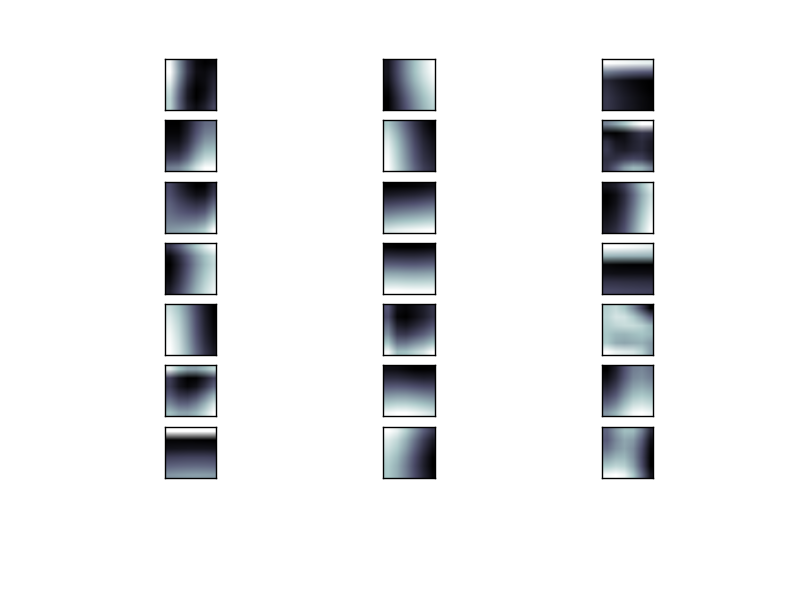
\includegraphics[height=10cm]{./spec_patch_clustersGMM21.png}
\caption{\label{fig:spec_patch_clustersGMM21}Spectrogram Patch GMM - 21 Clusters}
\end{figure}




\begin{verbatim}
import matplotlib.pyplot as plt
import matplotlib.cm as cm
import numpy as np
from sklearn.cluster import MeanShift, estimate_bandwidth

spec_patch = np.load('../data/1spec_patch.npy')
X = spec_patch.reshape(spec_patch.shape[0],6*6)
for bandwidth in [16,8,4,2,1,.5,.25,.125]:
    ms = MeanShift(bandwidth=bandwidth, bin_seeding=True)
    ms.fit(X)
    labels = ms.labels_
    cluster_centers = ms.cluster_centers_
    labels_unique = np.unique(labels)
    n_clusters_ = len(labels_unique)
    print "number of estimated clusters : %d" % n_clusters_
    num_rows = n_clusters_/3+1
    if n_clusters_ < 3:
        num_cols = n_clusters_+1
    else:
        num_cols = 3
    fig = plt.figure()
    plt.title('Mixture Components')
    for j in xrange(n_clusters_):
        plt.subplot(num_rows,num_cols,j+1)
        plt.imshow(cluster_centers[j].reshape(6,6),
                   cmap=cm.bone)
        frame = plt.gca()
        frame.axes.get_xaxis().set_visible(False)
        frame.axes.get_yaxis().set_visible(False)
    plt.savefig('spec_patch_clustersMeanShift%d%2f.png' % (n_clusters_,bandwidth))
\end{verbatim}


Now, we see that these pick up on the edge structure of the
spectrogram quite nice, just as we would expect.  Our next question is
where these are coming from in the spectrogram, we show this in
\ref{1S_spec_patch.png}, the blue denotes areas where no patches have
been extracted, the colors give a sense of how the extraction process
picks up on loud and quiet parts of the spectrogram.


\begin{verbatim}
import matplotlib.pyplot as plt
import numpy as np
S = np.load('../data/1S.npy')
spec_patch_ones = np.load('../data/1spec_patch_ones.npy')
S -= S.min()
S /= S.max()
S *= spec_patch_ones
plt.imshow(S[::-1],interpolation='nearest',aspect=3)
plt.xticks(np.arange(7)*100,tuple(str(i*100/5) for i in xrange(7)))
# since 8*16000 (sample rate)/512 (fft length) = 250
plt.yticks(np.arange(6)*8,tuple(str(i*250) for i in xrange(6))[::-1])
plt.xlabel('time (ms)')
plt.ylabel('freq (Hz)')
plt.savefig('1S_spec_patch.png')
\end{verbatim}

\begin{figure}[htb]
\centering
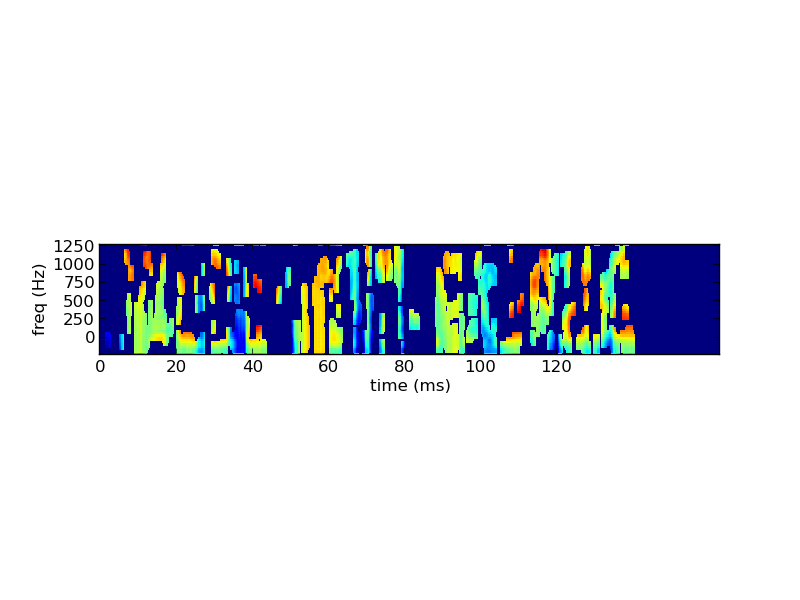
\includegraphics[height=10cm]{./1S_spec_patch.png}
\caption{\label{fig:1S_spec_patch}Example utterance Spectrogram - Edge Patch Locations}
\end{figure}


We then consider what happens when we apply the bernoulli clustering
algorithm (with EM) to the binary features.  A single utterance gives
us a fair sampling of the patches.
\subsection{Clustering over many parts}
\label{sec-2-2}

 
   From 28 utterances we extract a total of 50,000 patches (again
   these are in the top 90th percentile of edges for the utterance)
   and we do clustering over these.  The clustering is over the binary
   edge maps for the patches.  We clustered with 10, 20, 30, 50, 80,
   and 100 cluster centers to get a sense of what different numbers of
   clusters mean.

   Bernoulli Mixture models in high dimensions estimate a probability mass
   function of the form

   $$\mathbb{P}(X) = \sum_{k=1}^K \pi_k \prod_{e,f,s} X_{e,f,s}^{p_{k,e,f,s}} (1-X_{e,f,s})^{p_{k,e,f,s}}   $$

   where $K$ is the number of components in the mixture so $k$ is the
   component identity, the index $e$ ranging over ${1,2,\ldots,8}$
   represents the edge orientation, $f$ is the frequency band, and $s$
   is the time.  In the case of patches $f$ is not absolute, but
   instead is relative to the lowest frequency band in the patch, as
   we do not treat patches extracted from the lower part of the
   spectrogram as being different from those extracted from a higher
   part of the spectrogram.  $s$ is also not an absolute time either
   but is also relative to when the patch begins. The patches range
   over five edge frequency bands and five edge time blocks. So $f\in [ 5 ]$
   and $s\in [ 5 ]$.

   We perform clustering using the EM algorithm.  When running the EM
   algorithm we compute `cluster affinities' $A_{i,k}$- which are for
   each mixture component $k$ of our mixture model we compute the
   probability that a given data point, $X_i$, was generated by that
   mixture component.  More formally, a given mixture model is
   specified by associated a latent `label' $Z_i$ with each datapoint
   $X_i$.  This label $Z_i\in [K]$ where $K$ is the number of
   components.  We model the binary variabels that make up a data
   point $X_i$ as conditionally independent bernoulli trials given the
   label $Z_i$.  The affinity is $\mathbb{P}(Z_i = k\mid X_i)$

   Our formula is

   $$ A_{i,k} =\frac{\pi_k\prod_{e,f,s} X_{i,e,f,s}^{p_{k,e,f,s}} (1-X_{i,e,f,s})^{p_{k,e,f,s}}  }
   {\sum_{k'=1}^K \pi_k\prod_{e,f,s} X_{i,e,f,s}^{p_{k',e,f,s}} (1-X_{i,e,f,s})^{p_{k',e,f,s}}  }$$

   We find that in our bernoulli mixture model that these affinities tend to be highly degenerate and either very close to 0
   or very close to 1.


\begin{verbatim}
import matplotlib.pyplot as plt
import matplotlib.cm as cm
from matplotlib import rc
import numpy as np
rc('text', usetex=True)
fig = plt.figure()
plt.title('CDFs over $\max_k P(Z_i=k\mid X_i = x_i)$')
for mix_id, num_mix in enumerate([10,20,30,50,80,100]):
    plt.subplot(2,3,mix_id+1)
    sorted_affinities= np.sort(np.load('../data/bm_affinities%d.npy' % num_mix).astype(np.float32).max(1))
    plt.plot(sorted_affinities,
             np.arange(sorted_affinities.shape[0])/float(len(sorted_affinities))
             )
    plt.title('Empirical cdf \nfor %d components' % num_mix)

plt.subplots_adjust(wspace=.5,hspace=.5)

plt.savefig('mixture_affinities_cdfs.png')
plt.close()
\end{verbatim}

We then see in \ref{fig:mixture_affinities_cdfs} that essentially
every data point is assigned to single component with overwhelming
probability.  The curves in those plots are of the function

$$ \left( \tau,
          \frac{|\{i\mid \max_k A_{i,k} < \tau \}|}{n}\right)$$ 

which is the empirical cumulative distribution function of the maximum
estimated affinities for the data points.


\begin{figure}[htb]
\centering
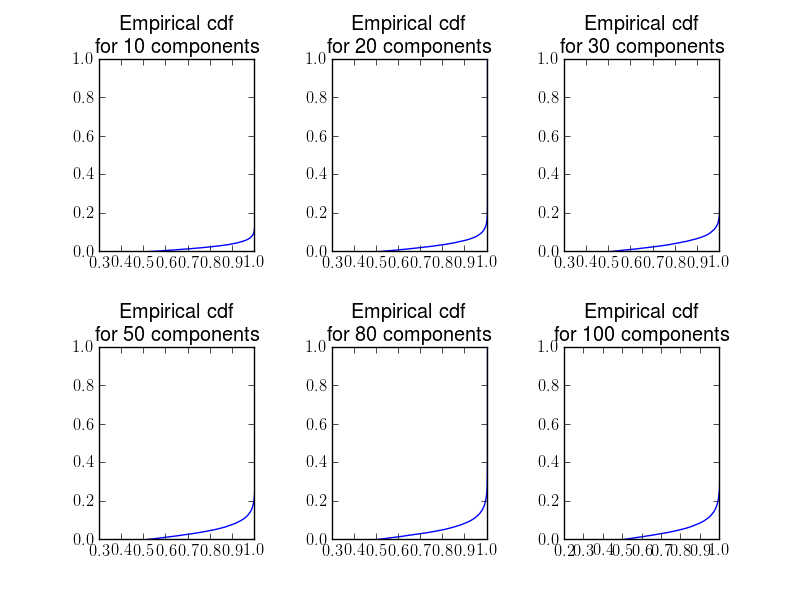
\includegraphics[height=10cm]{./mixture_affinities_cdfs.png}
\caption{\label{fig:mixture_affinities_cdfs}Empirical CDFs for the Max Component Affinities}
\end{figure}

The consequence of the fact that the affinities are degenerate is that
essentially the bernoulli mixture modeling provides a hard clustering
of the extracted patches.

We can then examine the cluster centers given by the templates, and,
more informatively, the affinities induce a clustering on the spectrogram
patches that gave rise to the bernoulli edge map features.  


\begin{verbatim}
import matplotlib.pyplot as plt
import matplotlib.cm as cm
from matplotlib import rc
import numpy as np
rc('text', usetex=True)
for num_mix in [10,20,30,50,80,100]:
    spec_avg_parts = np.load('../data/spec_avg_parts%d.npy' % num_mix)
    fig = plt.figure()
    for i in xrange(num_mix):
        plt.subplot((num_mix-1)/4+1,min(num_mix+1,4),i+1)
        plt.imshow(spec_avg_parts[i],cmap=cm.bone,interpolation='nearest')
        frame = plt.gca()
        frame.axes.get_xaxis().set_visible(False)
        frame.axes.get_yaxis().set_visible(False)
    plt.savefig('spec_avg_parts_%d.png' % num_mix)
\end{verbatim}


\begin{figure}[htb]
\centering
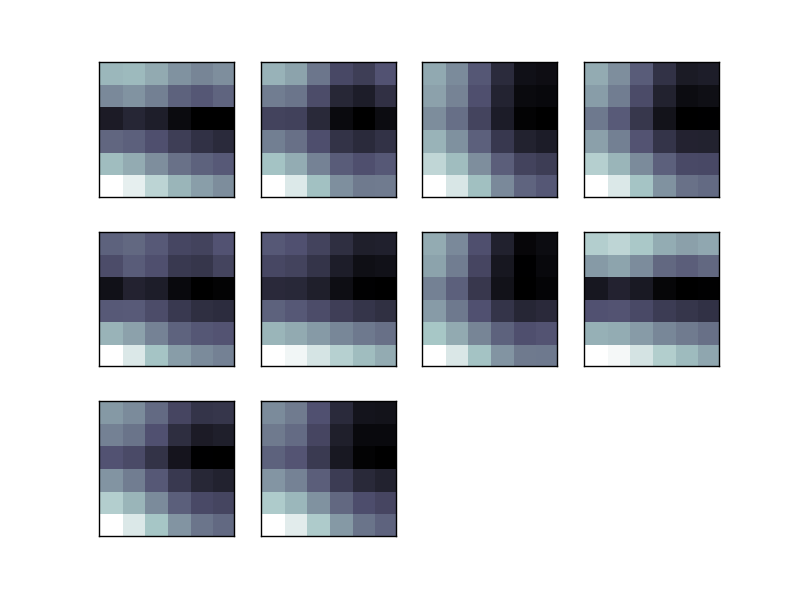
\includegraphics[height=10cm]{./spec_avg_parts_10.png}
\caption{\label{fig:spec_avg_parts_10}Spectrogram Part Clusters - 10 components}
\end{figure}

\begin{figure}[htb]
\centering
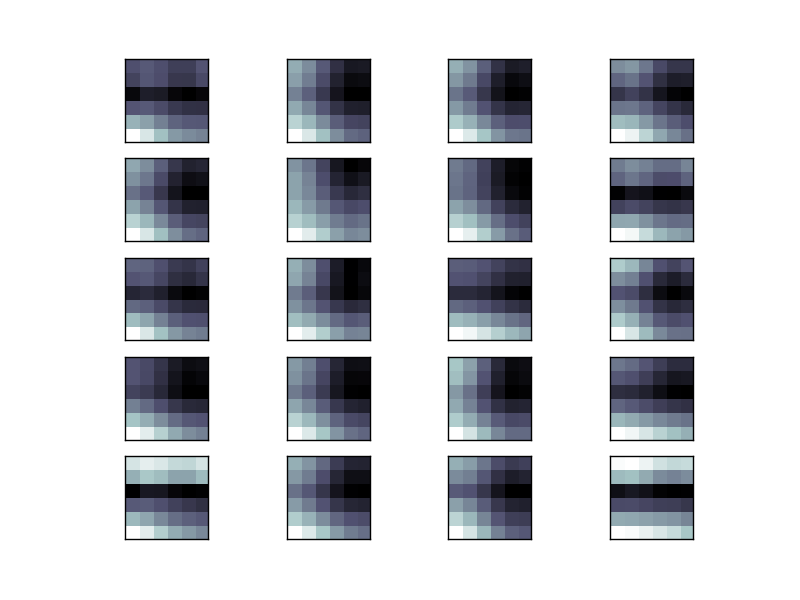
\includegraphics[height=11cm]{./spec_avg_parts_20.png}
\caption{\label{fig:spec_avg_parts_20}Spectrogram Part Clusters - 20 components}
\end{figure}

\begin{figure}[htb]
\centering
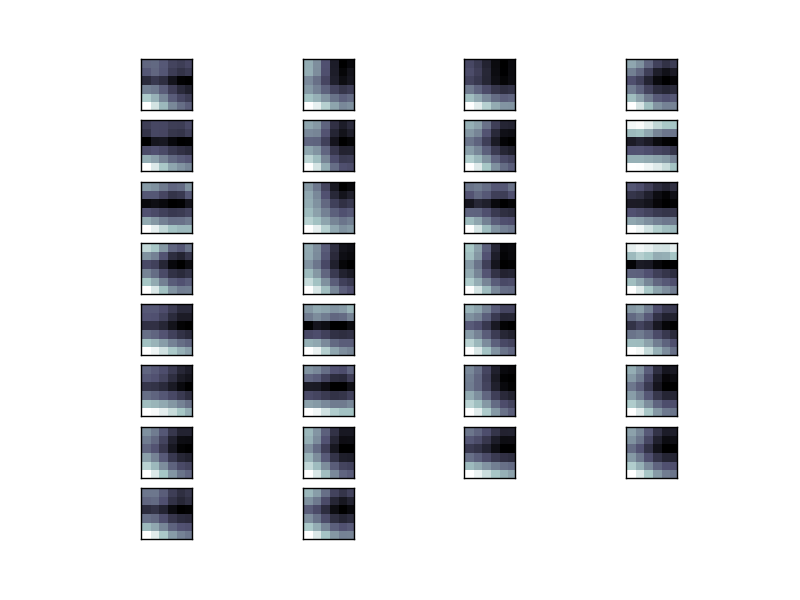
\includegraphics[height=12cm]{./spec_avg_parts_30.png}
\caption{\label{fig:spec_avg_parts_30}Spectrogram Part Clusters - 30 components}
\end{figure}

\begin{figure}[htb]
\centering
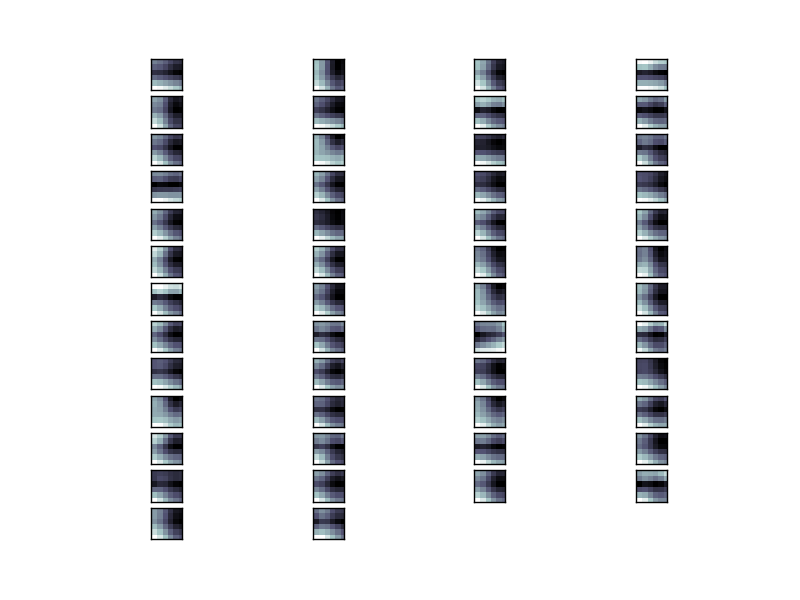
\includegraphics[height=14cm]{./spec_avg_parts_50.png}
\caption{\label{fig:spec_avg_parts_50}Spectrogram Part Clusters - 50 components}
\end{figure}

\begin{figure}[htb]
\centering
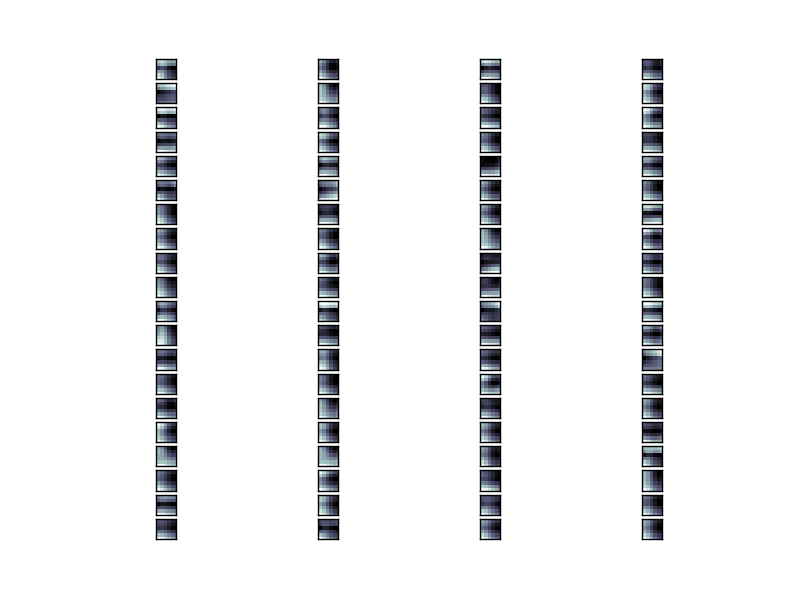
\includegraphics[height=16cm]{./spec_avg_parts_80.png}
\caption{\label{fig:spec_avg_parts_80}Spectrogram Part Clusters - 80 components}
\end{figure}

\begin{figure}[htb]
\centering
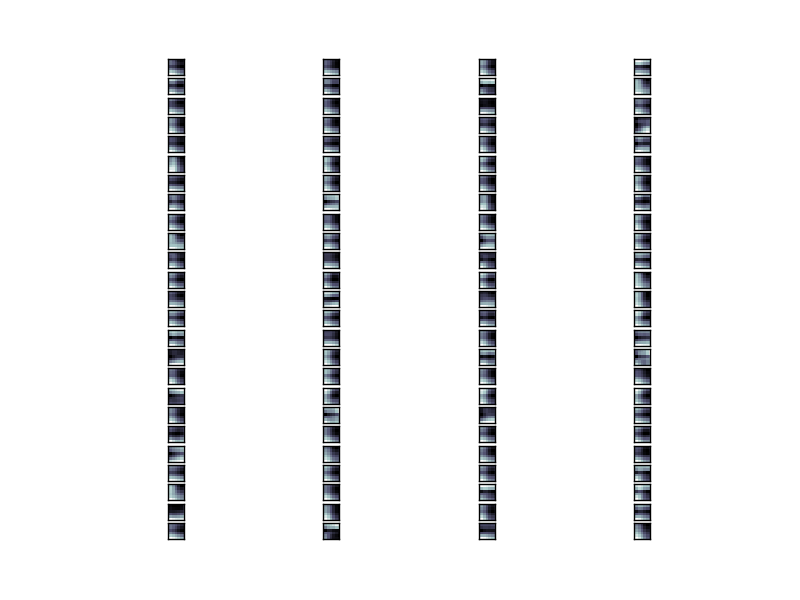
\includegraphics[height=20cm]{./spec_avg_parts_100.png}
\caption{\label{fig:spec_avg_parts_100}Spectrogram Part Clusters - 100 components}
\end{figure}


We also want to see what the parts are when we use a single utterance.
There is a noticeable lack of parts for vertical objects, whereas this
was observed in Waliji's experiment based on the figures provided.


\begin{verbatim}
import matplotlib.pyplot as plt
import matplotlib.cm as cm
from matplotlib import rc
import numpy as np
num_mix =20
spec_avg_parts = np.load('../data/1spec_avg_parts%d.npy' 
                         % num_mix)
fig = plt.figure()
for i in xrange(num_mix):
    plt.subplot((num_mix-1)/4+1,min(num_mix+1,4),i+1)
    plt.imshow(spec_avg_parts[i],cmap=cm.bone,interpolation='nearest')
    frame = plt.gca()
    frame.axes.get_xaxis().set_visible(False)
    frame.axes.get_yaxis().set_visible(False)
plt.savefig('1spec_avg_parts_%d.png' % num_mix)
\end{verbatim}

Even with only 2600 patches we see roughly the same patterns as we do
with many more patches as in \ref{1spec_avg_parts_20}.

\begin{figure}[htb]
\centering
\includegraphics[height=10cm]{./1spec_avg_parts_20.png}
\caption{\label{fig:1spec_avg_parts_20}Spectrogram Part Clusters - 20 components, 1 Utterance}
\end{figure}

The apparent lack of time-edges, that is, edges where the gradient is
zero across frequency bands but large between successive time points,
is likely going to be problematic for classification.  A useful
statistic to compute is in what clusters are those vertical edges
being assigned?  Additionally, one question is whether vertical edge
structure preserved under the feature map?  There are a couple of
approaches to answering these questions:
\begin{itemize}
\item cluster assignment inspection: among those patches that we declare
  non-background, how does the number of time edges correlate with cluster
  assignment.  Are time-edge heavy patches assigned to many different clusters
  or are they assigned to a particular set.
\item Time edges usually indicate broad-band noise (this is also something to verify)
  about the speech signal, we should note when those occur versus when they don't
  how that correlates to the patches
\item we should see if the patches with the most time-edges are unfairly penalized
  in that they tend to have fewer edges of the other types, and hence get ignored
\item we should also see what the classification performance of using these feature maps
  are, in particular, does the presence of time edges correlate with our
  misclassifications?
\end{itemize}
\subsubsection{Cluster Mapping}
\label{sec-2-2-1}


In order to do the cluster mapping process and get a proper feature
map, we take as input an edge map $E(t,f,e)\in \{0,1\}$ and we construct
a feature map $\Phi(t,f)\in \{-1,0,\ldots,num\_parts-1\}$ where
$num\_parts$ is the number of parts in our system.  $-1$ denotes background
and $0,\dots,num\_parts-1$ denote the indices for the part that is chosen.

It is important to note that while the edge map $E(t,f,e)$ is a coding over particular
time-frequency regions whether a particular edge type is present,
the feature map $\Phi(t,f)$ is a coding over regions of the edge map, in particular
its over the region $[t,t+part\_width) \times [f,f+part\_height)$ and over all edge
types.  Since we model the edge map features as conditionally independent bernoullis
the coding follows the formula:

$$ \underset{k}{\arg\max} \sum_{s\in[0,part\_width),g\in[0,part\_height],e} 
             E(t+s,f+g,e)\log p_{k,s,g,e} +(1 - E(t,f,e))\log (1-p_{k,s,g,e}).$$

We only perform this feature transformation on patches with sufficient edge activity:

$$ \sum_{s\in[0,part\_width),g\in[0,part\_height],e} 
             E(t+s,f+g,e) \geq \tau_{.9},$$

i.e. time-frequency regions where the edge activity is greater than
the 90$th$ percentile.  We can then think of a coding induced on the
spectrogram by doing this.  Namely, for non-background patch $b$ with
part code $k$ whose root location is at $(t,f)$ we construct a kernel
$\eta_b$ such that $\eta_b(t+s,f+g) = spec\_patch_k$ where
$spec\_patch_k$ is the average over the implicitly clustered
spectrogram clustering induced by the bernoulli model clustering.



\begin{verbatim}
import matplotlib.pyplot as plt
import matplotlib.cm as cm
import numpy as np
plt.figure()
plt.subplot(4,1,1)
S = np.load('../data/1S.npy')
plt.imshow(S[::-1],interpolation='nearest',aspect=3)
plt.xticks(np.arange(7)*100,tuple(str(i*100/5) for i in xrange(7)))
# since 8*16000 (sample rate)/512 (fft length) = 250
plt.yticks(np.arange(6)*8,tuple(str(i*250) for i in xrange(6))[::-1])
plt.xlabel('time (ms)')
plt.ylabel('freq (Hz)')

for code_id,num_parts in enumerate([15,20,25]):
    plt.subplot(4,1,code_id+2)
    S_coded = np.load('../data/1S_coded%d.npy' % num_parts)
    plt.imshow(S_coded[::-1],cmap=cm.bone,interpolation='nearest',aspect=3)
    plt.title('S coded with %d parts' %num_parts)
    plt.xticks(np.arange(7)*100,tuple(str(i*100/5) for i in xrange(7)))
    # since 8*16000 (sample rate)/512 (fft length) = 250
    plt.yticks(np.arange(6)*8,tuple(str(i*250) for i in xrange(6))[::-1])
    plt.xlabel('time (ms)')
    plt.ylabel('freq (Hz)')

plt.subplots_adjust(hspace=1,left=0)
plt.savefig('1S_coded_compare.png')


plt.figure()
plt.subplot(4,1,1)
S = np.load('../data/1S.npy')
plt.imshow(S[::-1],interpolation='nearest',aspect=3)
plt.xticks(np.arange(7)*100,tuple(str(i*100/5) for i in xrange(7)))
# since 8*16000 (sample rate)/512 (fft length) = 250
plt.yticks(np.arange(6)*8,tuple(str(i*250) for i in xrange(6))[::-1])
plt.xlabel('time (ms)')
plt.ylabel('freq (Hz)')

for code_id,num_parts in enumerate([15,20,25]):
    plt.subplot(4,1,code_id+2)
    S_coded = np.load('../data/1S_coded%d.npy' % num_parts)
    plt.imshow(S_coded[::-1],interpolation='nearest',aspect=3)
    plt.title('S coded with %d parts' %num_parts)
    plt.xticks(np.arange(7)*100,tuple(str(i*100/5) for i in xrange(7)))
    # since 8*16000 (sample rate)/512 (fft length) = 250
    plt.yticks(np.arange(6)*8,tuple(str(i*250) for i in xrange(6))[::-1])
    plt.xlabel('time (ms)')
    plt.ylabel('freq (Hz)')

plt.subplots_adjust(hspace=1,left=0)
plt.savefig('1S_coded_compare_color.png')
\end{verbatim}


\begin{figure}[htb]
\centering
\includegraphics[height=15cm]{./1S_coded_compare_color.png}
\caption{\label{fig:1S_coded_compare}Spectrogram Coding Comparison}
\end{figure}



The next step is to visualize what happens when we denoise or code a
spectrogram using the parts.  We take the estimated templates from the
EM algorithm and we are going to use these to code spectrograms.  The
step is going

\end{document}
